\documentclass{exam}
\usepackage[utf8]{inputenc}
\usepackage{upgreek}
\usepackage[margin=1in]{geometry}
\usepackage{amsmath,amssymb}
\usepackage{multicol}
\usepackage{stmaryrd}
\usepackage{graphicx}
\usepackage{caption}
\usepackage{tikz}
\usepackage{dsfont}
\usepackage{enumitem}
\usepackage{hyperref}
\usetikzlibrary{matrix}
\newcommand\tab[1][1cm]{\hspace*{#1}}
\pagestyle{head}
\firstpageheader{}{}{}
\runningheader{\examnum}{\class}{\name}
\runningheadrule
\newcommand{\class}{Fundamentos de bases de datos}
\newcommand{\term}{Facultad de Ciencias UNAM}
\newcommand{\examnum}{Practica 01 - Bitácora}
\newcommand{\examdate}{07/03/2022}
\newcommand{\name}{Ernesto Cárdenas Torres - 306155406}

\begin{document}

\noindent
\begin{tabular*}{\textwidth}{l @{\extracolsep{\fill}} r @{\extracolsep{6pt}} l}
\textbf{\class} & \textbf{\term}\\
\textbf{\examnum} & \textbf{\name}\\
\textbf{\examdate}
\end{tabular*}\\
\rule[2ex]{\textwidth}{2pt}

\section*{Bitácora}

\subsection*{Sistema operativo y versión}

Memoria: 11.4GiB
Procesador: Intel Core i5-4300M CPU @ 2.60GHz x 4
SO: Linux
Gnome 3.38
Kernel: 5.10.0-11-amd64
Arch: 64 bits

\subsection*{Distribución}

Debian 11 - Bullseye

\subsection*{Versión de la instalación}

PostgreSQL Debian 14.2-1.pgdg110+1

\subsection*{Tiempo requerido}

15 minutos

\subsection*{Explicación del paso a paso}

\begin{enumerate}
    \item Agregamos GPG key de PostgreSQL y PGAdmin4
    
    \begin{figure}[h]
        \centering
        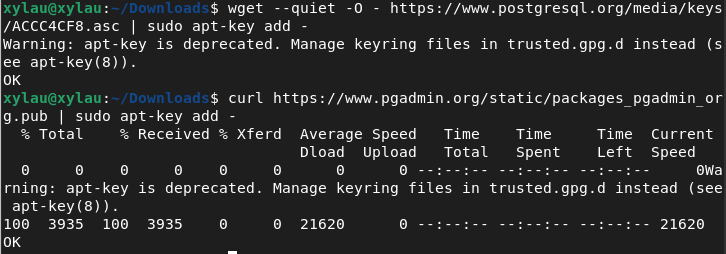
\includegraphics[width = 15cm]{imgCardenas/1.png}
    \end{figure}
    
    \item Agregamos repositorios y hacemos update
    
    \begin{figure}[h]
        \centering
        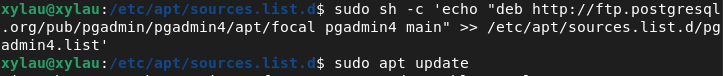
\includegraphics[width = 15cm]{imgCardenas/2.png}
    \end{figure}
    \newpage
    \item Verificamos instalación
    
    \begin{figure}[ht]
        \centering
        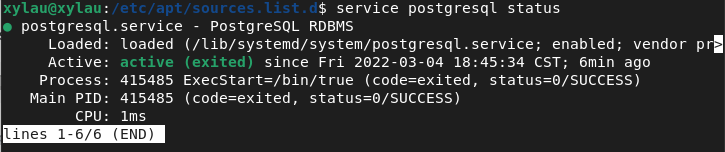
\includegraphics[width = 15cm]{imgCardenas/3.png}
    \end{figure}
    
    \item Nos conectamos y abrimos el prompt
    
    \begin{figure}[h!]
        \centering
        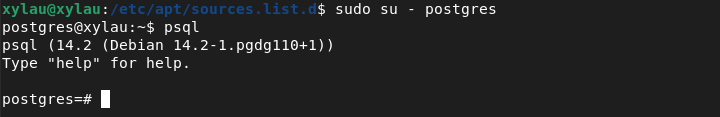
\includegraphics[width = 15cm]{imgCardenas/4.png}
    \end{figure}
    
    \item Cambiamos la pass del Super User
    
    \begin{figure}[h!]
        \centering
        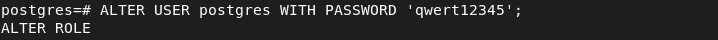
\includegraphics[width = 15cm]{imgCardenas/5.png}
    \end{figure}
    
\end{enumerate}


\subsection*{Comentarios y problemas}

La instalación fue sencilla, solo se encontró conflicto al querer hacer copy \& paste desde el pdf a la terminal, porque el pdf siempre cambia los símbolos.


\end{document}
